\section{Apprentissage machine}
  \subsection{Principe de base}
    Selon l'\ac{OQLF}\parencite{OQLF:ApprentissageProfond:2024}, la définition de l'apprentissage profond est la suivante:
    \begin{definition}
    Mode d'apprentissage automatique généralement effectué par un réseau de neurones artificiels composé de plusieurs couches de neurones hiérarchisées selon le degré de complexité des concepts, et qui, en interagissant entre elles, permettent à un agent d'apprendre progressivement et efficacement à partir de mégadonnées.
    \end{definition}
    D'un point de vue mathématique, l'apprentissage est obtenu en représentant les données sous forme matricielle ou vectorielles et en les soummettant à plusieurs opérations algébriques simples successivement de manière à ce que le code produise une sortie désirée. Le problème est formulé non pas en demandant à ce que le logiciel performe des opérations spécifiques, mais en spécifiant une architecture de réseau et un ensemble de pondérations à modifier pour minimiser une foncion de perte donnée.
  \subsection{Le pipeline d'apprentissage machine}
  \subsubsection{Survol}
      Cette section va décrire le processus utilisé pour obtenir des résultats dans le champs de l'apprentissage machine. Ce processus est souvent appelé \og{pipeline d'apprentissage machine} \fg{}. Il est décliné en 6 étapes:
        \begin{enumerate}
          \item Préparation des données
          \item Ingénierie des caractéristiques
          \item Développement du réseau et entrainement
          \item Évaluation des résultats et amélioration du modèle
          \item Déploiement et suivi
        \end{enumerate}
      Les sections suivantes détailleront les opérations à chaque étape
    \subsubsection{Collection et préparation des données}
        La préparation des données consiste à prendre un ensemble de données et au besoin le nettoyer, enlever les données abérantes, de mettre à l'échelle les données et la création d'un ensemble de données d'apprentissage et d'un ensemble de validation.
    \subsubsection{Ingénierie des caractéristiques}
      L'ingénierie des caractéristiques consiste à créer des variables intermédiaires, catégoriques ou de traiter les données de manière à améliorer la capacité prédicitive du modèle d'apprentissage machine dans l'extraction des données pertinentes.
    \subsubsection{Sélection, codage et entrainement du modèle}
      Cette partie du \og{pipeline} \fg{} est le coeur de l'opération. À cette étape, une méthode d'extraction des données est choisie et implémentée. Le modèle peut être un modèle personalisé ou issue de la littérature ou d'une librairie pré construite. Deux méthodes sont potentiellement applicables à l'apprentissage. Un modèle pré-existant, avec ses pondération peut être appliqué à un nouveau problème en utilisant de l'apprentissage de transfert (\og{Transfer Learning} \fg{} en anglais) ou le modèle peut être entrainé à partir de pondérations initiales aléatoires. L'apprentissage itère au travers de l'ensemble de données en mettant les données en lots (\og{Batch} \fg{} en anglais) et en modifiant les pondération de manière à minimiser la fonction de pertes. À chaque fois que le modèle complète une itération au travers de l'ensemble des données, une époque (\og{epoch} \fg{} en anglais) est dite complétée. La plupart du temps, la fonction de perte utilisée est compilée pour l'ensemble d'entrainement et de validation à la fin de chaque époque pour permettre d'évaluer la convergence du modèle, ainsi que le degré de sur-ajustement potentiel du modèle. Un modèle est dit sur-ajusté s'il prédit bien sur l'ensemble d'appentissage mais mal sur l'ensemble de validation. Dans certains, la vitesse de prédiction où la taille des modèles peut-être un facteur limitant si le modèle doit être implémentée sur un appareil mobile ou sur des applications temps réel.
    \subsubsection{Évaluation du modèle}
      Une fois l'apprentissage completé, le modèle peut-être évalué de différentes manières. Plusieurs indicateurs mesurent le degré de précision du modèle, la vitesse de sa convergence peuvent être évalués en fonction de l'utilisation désirée du modèle. En vision numérique, le degré de similarité entre les données d'apprentissage annotées et les prédictions est souvent la métrique d'évaluation de prédilection.
    \subsubsection{Déploiement et suivi}
      À cette étape, le modèle est deployé. Le suivi consiste principalement à recenser les comportement abhérants du modèle et les réintégrer dans le modèle au besoin. 
  \subsection{Principe de base des réseaux de neurones}
  Le principe de base des réseaux de neurones et qu'en implémentant de multiples couches de fonction linéaires couplées avec des fonctions d'activation, il est possible de reproduire des tâches ou fonctions complexes. 
    \subsubsection{Le neurone}
      Chaque neurone dans un réseau est une opération algébrique avec une fonction d'activation:

        \begin{figure}[!h]
          \centering
          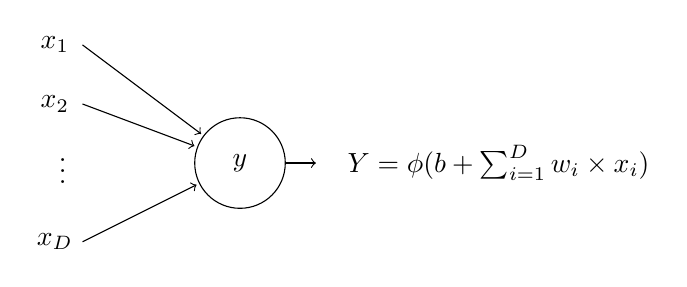
\begin{tikzpicture}[shorten >=1pt,->]
            \tikzstyle{unit}=[draw,shape=circle,minimum size=1.15cm]
            \node[unit](p) at (2,1){$y$};
            \node(dots) at (-0.25,1){\vdots};
            \draw (0,2.5) node[xshift=-10]{$x_1$} --(p);
            \draw (0,1.75) node[xshift=-10]{$x_2$} --(p);
            \draw (0,0) node[xshift=-10]{$x_D$} -- (p);
            \draw (p) -- (3,1) node[xshift=65]{$Y = \phi(b  + \sum_{i=1}^{D} w_i \times x_i)$};
          \end{tikzpicture}
          \caption{Un neurone dans un réseau de neurone}
          \label{fig:neurone}
         % https://davidstutz.de/illustrating-convolutional-neural-networks-in-latex-with-tikz/
        \end{figure}
      La fonction $\phi $ est une fonction d'activation qui sera détaillée dans la section \ref{sssection:activ_fn}.
      \FloatBarrier
    \subsubsection{Réseau de neurones simple}
      Un réseau de neurone arrange plusieurs neurones en série ou en parallèle où les pondérations sont altérées pour permettre de faire des tâches variant en complexité. Une couche est un ensemble de neurones qui est le résultat d'un même nombre d'opérations algébriques. Les différentes couches peuvent avoir des nombres de neurones variables. La couche entrante est le premier ensemble de données qui est fourni au réseau et la couche sortante est la dernière couche de neurones en sortie à l'analyste. La figure \ref{fig:perceptron} montre une architecture hypothétique de réseau de neurones.\par
      \begin{figure}[!h]
        \centering
          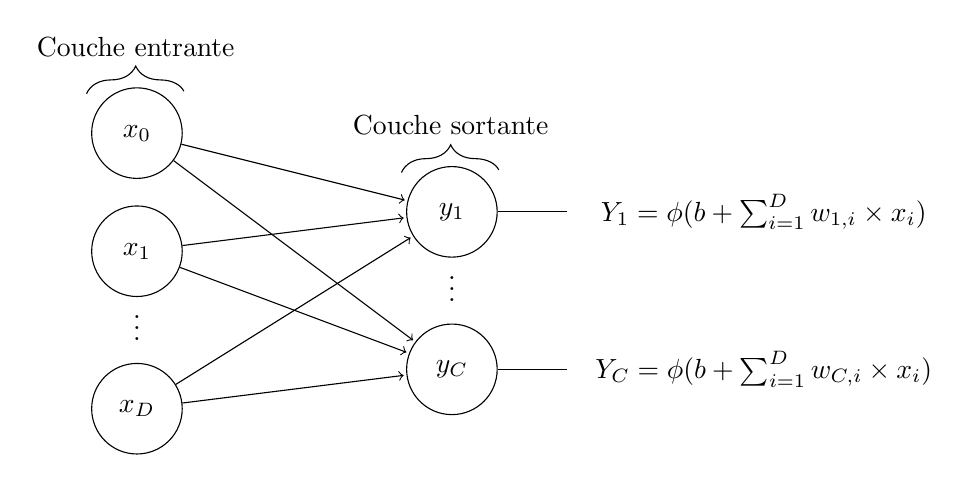
\begin{tikzpicture}[shorten >=1pt]
            \tikzstyle{unit}=[draw,shape=circle,minimum size=1.15cm]
    
            \node[unit](x0) at (0,3.5){$x_0$};
            \node[unit](x1) at (0,2){$x_1$};
            \node(dots) at (0,1.125){\vdots};
            \node[unit](xd) at (0,0){$x_D$};
    
            \node[unit](y1) at (4,2.5){$y_1$};
            \node(dots) at (4,1.625){\vdots};
            \node[unit](yc) at (4,0.5){$y_C$};
            \draw (y1) -- (5.5,2.5) node[xshift=70]{$Y_1 = \phi(b + \sum_{i=1}^{D} w_{1,i} \times x_i)$};
            \draw (yc) -- (5.5,0.5) node[xshift=70]{$Y_C = \phi(b + \sum_{i=1}^{D} w_{C,i} \times x_i)$};
    
            \draw[->] (x0) -- (y1);
            \draw[->] (x0) -- (yc);
    
            \draw[->] (x1) -- (y1);
            \draw[->] (x1) -- (yc);
    
            \draw[->] (xd) -- (y1);
            \draw[->] (xd) -- (yc);
    
            \draw [decorate,decoration={brace,amplitude=10pt},xshift=-4pt,yshift=0pt] (-0.5,4) -- (0.75,4) node [black,midway,yshift=+0.6cm]{Couche entrante};
            \draw [decorate,decoration={brace,amplitude=10pt},xshift=-4pt,yshift=0pt] (3.5,3) -- (4.75,3) node [black,midway,yshift=+0.6cm]{Couche sortante};
          \end{tikzpicture}
          % https://davidstutz.de/illustrating-convolutional-neural-networks-in-latex-with-tikz/
        \caption{Réseau de neurones à couche simple}
        \label{fig:perceptron}
      \end{figure}
      Le réseau montré à la figure \ref{fig:perceptron} est dit pleinement connecté si sa valeur est une somme pondérée de l'ensemble des couches précédentes. 
      \FloatBarrier
    \subsubsection{Réseau de neurones multicouches}
      Plusieurs couches dites \og{cachées} \fg{} peuvent être ajoutées entre l'entrée et la sortie du réseau de neurones pour permettre de traiter des problèmes plus ou moins complexes. L'enjeu comporte cependant des compromis puisque l'ajout de couches ajoute des paramètre à ajuster, augmentant la taille du modèle. D'autre part, plus le nombre de paramètres est grand, plus la contribution d'une pondération est petite. Ce problème est nommé le problème de \og{disparition de gradient} \fg{} dans la littérature.
      \begin{figure}[!h]
        \centering
          \begin{tikzpicture}[shorten >=1pt]
            \tikzstyle{unit}=[draw,shape=circle,minimum size=1.15cm]
    
            \node[unit](x00) at (-1,3.5){$x_0$};
            \node[unit](x01) at (-1,2){$x_1$};
            \node(dots) at (-1,1.125){\vdots};
            \node[unit](x0d) at (-1,0){$x_{N_0}$};

            \node[unit](y11) at (1,4.5){$y_1^{(1)}$};
            \node[unit](y12) at (1,3){$y_2^{(1)}$};
            \node(dots1) at (1,1.125){\vdots};
            \node[unit](y1n) at (1,-1){$y_{N_1}^{(1)}$};

            \node(middots1) at (3,4.5){$\ldots$};
            \node(middots2) at (3,2.5){$\ldots$};
            \node(middots3) at (3,1){$\ldots$};

            \node[unit](yc-11) at (5,4.5){$y_1^{(C-1)}$};
            \node[unit](yc-12) at (5,2){$y_2^{(C-1)}$};
            \node(dotsc) at (5,0.125){\vdots};
            \node[unit](yc-1n) at (5,-2){$y_{N_{C-1}}^{(C-1)}$};

            \node[unit](yc1) at (8,2.5){$y^{(C)}_1$};
            \node(dotsn) at (8,1.625){\vdots};
            \node[unit](ycn) at (8,0.5){$y^{(C)}_{N_{C}}$};
            \draw (yc1) -- (9.5,2.5) node[right]{$Y^{(C)}_{1} = \phi(b_k + \sum_{i=1}^{N_{C-1}} w^{(C)}_{1,i} \times y^{(C-1)}_i)$};
            \draw (ycn) -- (9,0.5) node[right]{$Y^{(C)}_{N_{C}} = \phi(b_{N_C} + \sum_{i=1}^{N_{C-1}} w^{(C)}_{N_{C},i} \times y^{(C-1)}_i)$};
    
            \draw[->] (x00) -- (y11);
            \draw[->] (x00) -- (y12);
            \draw[->] (x00) -- (y1n);
    
            \draw[->] (x01) -- (y11);
            \draw[->] (x01) -- (y12);
            \draw[->] (x01) -- (y1n);
    
            \draw[->] (x0d) -- (y11);
            \draw[->] (x0d) -- (y12);
            \draw[->] (x0d) -- (y1n);

            \draw[->,path fading=east] (y11) -- (middots1);
            \draw[->,path fading=east] (y12) -- (middots1);
            \draw[->,path fading=east] (y1n) -- (middots1);

            \draw[->,path fading=east] (y11) -- (middots2);
            \draw[->,path fading=east] (y12) -- (middots2);
            \draw[->,path fading=east] (y1n) -- (middots2);

            \draw[->,path fading=east] (y11) -- (middots3);
            \draw[->,path fading=east] (y12) -- (middots3);
            \draw[->,path fading=east] (y1n) -- (middots3);

            \draw[->,path fading=west] (middots1) -- (yc-11);
            \draw[->,path fading=west] (middots1) -- (yc-12);
            \draw[->,path fading=west] (middots1) -- (yc-1n);

            \draw[->,path fading=west] (middots2) -- (yc-11);
            \draw[->,path fading=west] (middots2) -- (yc-12);
            \draw[->,path fading=west] (middots2) -- (yc-1n);

            \draw[->,path fading=west] (middots3) -- (yc-11);
            \draw[->,path fading=west] (middots3) -- (yc-12);
            \draw[->,path fading=west] (middots3) -- (yc-1n);

            \draw[->] (yc-11) -- (yc1);
            \draw[->] (yc-11) -- (ycn);

            \draw[->] (yc-12) -- (yc1);
            \draw[->] (yc-12) -- (ycn);

            \draw[->] (yc-1n) -- (yc1);
            \draw[->] (yc-1n) -- (ycn);
    
            \draw [decorate,decoration={brace,amplitude=10pt},xshift=-4pt,yshift=0pt] (-1.5,5.5) -- (-0.25,5.5) node [black,right,xshift=-0.8cm,yshift=+0.4cm,rotate=45]{Couche entrante};
            \draw [decorate,decoration={brace,amplitude=10pt},xshift=-4pt,yshift=0pt] (0.5,5.5) -- (1.75,5.5) node [black,right,xshift=-0.8cm,yshift=+0.4cm,rotate=45]{Couche cachée 1};
            \draw [decorate,decoration={brace,amplitude=10pt},xshift=-4pt,yshift=0pt] (4.5,5.5) -- (5.75,5.5) node [black,right,xshift=-0.8cm,yshift=+0.4cm,rotate=45]{Couche cachée C-1};
            \draw [decorate,decoration={brace,amplitude=10pt},xshift=-4pt,yshift=0pt] (7.5,5.5) -- (8.75,5.5) node [black,right,xshift=-0.8cm,yshift=+0.4cm,rotate=45]{Couche sortante};
          \end{tikzpicture}
          % https://davidstutz.de/illustrating-convolutional-neural-networks-in-latex-with-tikz/
        \caption{Réseau de neurones à couches multiples}
        \label{fig:multi_layer_perceptron}
      \end{figure}
      \FloatBarrier
  \subsection{Opérations communes dans l'apprentissage machine}
    \subsubsection{La fonction de perte}
      La fonction de perte de perte est la fonction objectif que le réseau de neurones essaie de minimiser. \textcite{Azad:LossFunctions:2023, Jadon:SurveyLoss:2020} donnent un survol des principaux types de fonction de pertes et de leur applicabilité pour différentes tâches de segmentation d'image. Le choix d'une fonction de perte est dépendant de la taille de l'objet à détecter et de l'équilibre entre les différentes classes à détecter:\par
      \paragraph{Entropie Croisée} L'entropie croisée est une mesure de la distance statistique entre deux ensembles et a été introduite par \textcite{Shannon:MathematicalTheory:1948}. Ici elle mesure la distance entre la prédiction du modèle et les annotations sur les données entrantes. Pour donner une distribution de probabilité, une fonction softmax est appliquée aux résultantes du réseau de neurones.
      Les équations \ref{eq:entropie_croisee}, \ref{eq:grnd_truth_vector} et \ref{eq:prob_class_vector} donnent la définition formelle de l'entropie croisée \parencite{Wallach:DeepLearning:2024}.\par
      \begin{align}
        EC & = -\frac{1}{I \times N} \sum_{n=1}^{N_{images}}\sum_{i=1}^{N_{pixels}}\sum_{j=1}^{N_{classes}}r^{n}_{ij} \log{p^{n}_{ij}} \label{eq:entropie_croisee}\\
        r^{n}_{ij} & = \begin{cases}
          1,& \mbox{si le pixel i de l'image n appartient à la classe j dans l'annotation d'entrainement}\\
          0,& \mbox{autrement}\\ \end{cases}\label{eq:grnd_truth_vector}\\
        p^{n}_{ij} & \in [0,1]\mbox{ est la prédiction du modèle concernant la catégorie j pour le pixel i}\label{eq:prob_class_vector}
      \end{align}
      $r^{n}_{ij}$ est la classe(j) annotée du pixel i de l'image n et $p^{n}_{ij}$ est la probabilité prédite par le modèle que le pixel i de l'image j appartienne à la classe j. La probabilité est obtenu en appliquant une fonction softmax aux sorties du modèle. 
      \paragraph{Entropie Croisée binaire} L'entropie croisée peut être utilisé pour un problème de classification binaire. Dans ce cas, il n'y a que 2 classes (vrai ou faux). L'entropie croisée binaire peut donc être représenté par les équations \ref{eq:entropie_croisee_binaire}, \ref{eq:grnd_truth_vector_ecb} et \ref{eq:prob_class_vector_ECB}
      \begin{align}
        ECB & = -\frac{1}{I \times N} \sum_{n=1}^{N_{images}}\sum_{i=1}^{N_{pixels}}r^{n}_{iV} \log{p^{n}_{iV}} +
        (1-r^{n}_{iV}) \log{(1-p^{n}_{iV})} \label{eq:entropie_croisee_binaire}\\
        r^{n}_{iV} & = \begin{cases}
          1,& \mbox{si le pixel i de l'image n appartient à la classe d'identification dans l'annotation d'entrainement}\\
          0,& \mbox{autrement}\\ \end{cases}\label{eq:grnd_truth_vector_ecb}\\
        p^{n}_{iV} & \in [0,1]\mbox{ est la probabilité que le pixel i appartienne à la classe identifiée}\label{eq:prob_class_vector_ECB}
      \end{align}
      \paragraph{Coefficient de Dice} 
      Le coefficient de Dice trouve ses origines dans les sciences de la nature \parencite{Dice:MeasuresAmount:1945} et est défini aux équations \ref{eq:DICE1} et \ref{eq:DICE2}.
      \begin{align} 
        CDS & = \frac{2 \times \lvert X \cap Y \rvert}{\lvert X \rvert + \lvert Y \rvert}\label{eq:DICE1} \\
        CDS & = \frac{2 \times VP}{2 \times VP + FP + FN}\label{eq:DICE2}
      \end{align}
    \subsubsection{Métriques pour l'évaluation}
      \paragraph{Indice de Jaccard} L'indice de Jaccard provient lui aussi des sciences de la nature \parencite{Jaccard:DistributionFlore:1901} et est plus communément utilisé comme fonction pour l'évaluation de différentes méthodes d'apprentissage. Il est très similaire au coefficient de Dice. L'indice de Jaccard est défini aux équations \ref{eq:IoU1} et \ref{eq:IoU2}. On réfère à cet indice sous le nom d'\ac{IoU} dans la plupart de la littérature. Il n'est pas utilisé comme fonction de perte puisqu'il n'est pas différentiable et ne se prête donc pas à la rétro-propagation.
      \begin{align} 
        IoU & = \frac{\lvert X \cap Y \rvert}{\lvert X \cup Y \rvert}\label{eq:IoU1} \\
        IoU & = \frac{VP}{VP + FP + FN}\label{eq:IoU2}
      \end{align}
      \paragraph{Justesse ou \og{Accuracy} \fg{}} 
      La justesse vise à quantifier le pourcentage de prédictions valides du modèle et est définie à l'équation \ref{eq:acc}\parencite{Wallach:DeepLearning:2024}.
      \begin{align}
        Justesse & = \frac{VP+VN}{VP + FP + FP + FN}\label{eq:acc}
      \end{align}
      \paragraph{Précision}
      La précision indique quel pourcentage des zones identifiées est valide et est définie à l'équation \ref{eq:prec}\parencite{Wallach:DeepLearning:2024}.
      \begin{align}
        Precision & = \frac{VP}{VP + FP}\label{eq:prec}
      \end{align}
      \paragraph{Rappel ou \og{Recall} \fg{}}
      La rappel indique quel pourcentage des zones positives n'ont pas été identifiées. Il est défini à l'équation \ref{eq:rappel}\parencite{Wallach:DeepLearning:2024}.
      \begin{align}
        Rappel & = \frac{VP}{VP + FN}\label{eq:rappel}
      \end{align}
      \paragraph{Score F1} Le Score F1 indique la capacité du modèle à faire un compromis entre la précision des prédictions et la capacité à ne pas manquer d'instances. Il est défini à l'équation 
      \begin{align}
        F1 & = \frac{2}{\frac{1}{Rappel} + \frac{1}{Precision}}\label{eq:F1_1}\\
        F1 & = \frac{VP}{VP + \frac{1}{2} (FN + FP)}
      \end{align}
    \subsubsection{Apprentissage et Rétro-propagation}
      La rétro-propagation a été introduite comme méthode pour modifier les pondérations des différents opérations algébriques par \textcite{Rumelhart:LearningRepresentations:1986}. La méthode consiste à créer une fonction cumulée d'erreur pour les extrants des réseaux neuronaux. Ensuite, des dérivées partielles sont calculées pour chaque neurones en amont pour trouver la modification requises pour minimiser la fonction d'erreur. Deux méthodes sont envisagées dans l'article initial. La première, modifie les pondérations après chaque donnée d'entrainement tandis que la deuxième somme les erreurs pour l'ensemble du jeu de données d'entrainement. Une troisième voie existe et est le plus souvent exploitée aujourd'hui qui consiste à calculer les modifications aux pondérations pour des lots de données qui sont des sous-ensemble de l'échantillon complet. En effet, le calcul des pondérations pour chaque échantillon créé des problèmes de stabilité et de convergence pour l'algorithme puisqu'un échantillons peut être à la limite de l'ensemble et créer un grande variation de paramètre mais l'évaluation des dérivées pour l'ensemble de l'échantillon peut être trop honéreux en termes de mémoire pour de grands échantillons \parencite{Wallach:DeepLearning:2024}.\par
      
      Soit une fonction d'erreur E, et le neurone $ y^{(C)}_1 $ de la figure \ref{fig:multi_layer_perceptron}. Il est possible trouver les variation de pondérations qui réduiraient l'erreur par l'équation \ref{eq:deriv_weights} comme le montre \textcite{Rumelhart:LearningRepresentations:1986}:
      \begin{align}
        x^{C}_k &= b_k + \sum_{i=1}^{N_{C-1}} w^{(C)}_{k,i} \times Y^{(C-1)}_i\\
        Y^{C}_k &= \phi(x^{C}_k)\\
        E &= \sum^{N_C}_{k=1} f(Y^{C}_k)\\
        \frac{\partial{E}}{\partial{w^{(C)}_{k,i}}}\bigg|_{w=\overrightarrow{w}_{t}} &= \frac{\partial{E}}{\partial{f(Y^{C}_k)}} \cdot \frac{\partial{f(Y^{C}_k)}}{\partial{w^{(C)}_{k,i}}}\\
        \frac{\partial{E}}{\partial{w^{(C)}_{k,i}}}\bigg|_{w=\overrightarrow{w}_{t}} &= \frac{\partial{E}}{\partial{f(Y^{C}_k)}} \cdot \frac{\partial{f(Y^{C}_k)}}{\partial{Y^{C}_k}} \cdot \frac{\partial{Y^{C}_k}}{\partial{w^{(C)}_{k,i}}} \\
        \frac{\partial{E}}{\partial{w^{(C)}_{k,i}}}\bigg|_{w=\overrightarrow{w}_{t}} &= \frac{\partial{E}}{\partial{f(Y^{C}_k)}} \cdot \frac{\partial{f(Y^{C}_k)}}{\partial{Y^{C}_k}} \cdot \frac{\partial{Y^{C}_k}}{\partial{x^{C}_k}} \cdot \frac{\partial{x^{C}_k}}{\partial{w^{(C)}_{k,i}}}\\
        \underbrace{\frac{\partial{E}}{\partial{w^{(C)}_{k,i}}}\bigg|_{w=\overrightarrow{w}_{t}}}_\text{Perte / poids} &= \underbrace{\frac{\partial{E}}{\partial{f(Y^{C}_k)}}}_\text{Perte / fn perte} \cdot \underbrace{\frac{\partial{f(Y^{C}_k)}}{\partial{Y^{C}_k}}}_\text{Fn perte / sortie activation} \cdot \underbrace{\frac{\partial{Y^{C}_k}}{\partial{x^{C}_k}}}_\text{Activation / fn lin.} \cdot \underbrace{Y^{(C-1)}_i}_\text{fn lin. / pond.}\label{eq:deriv_weights}
      \end{align}
    Dans son implémentation la plus simple, un vecteur de l'ensemble des dérivées partielles $\nabla{w_{t}} = \left[ \frac{\partial{E}}{\partial{w^{(1)}_{1,1}}} \ldots \frac{\partial{E}}{\partial{w^{(C)}_{k,i}}} \right] $ est multiplié par un paramètre fixe et ajouté au paramètres actuels $\overrightarrow{w}_{t} = \left[w^{(1)}_{1,1} \ldots w^{(C)}_{k,i}  \right] $. Les pondérations pour la prochaine itération donc $\overrightarrow{w}_{t+1} = \overrightarrow{w}_{t} - \varepsilon \cdot \nabla{w_{t}} $. Dans les méthodes modernes, des paramètres d'inertie et de vitesses sont ajoutés pour améliorer la stabilité des algorithmes. La section \ref{ssec:grad_desc} détaillera les algorithmes de descente de gradient les plus communs. Il est important de noter que ces méthodes n'utilisent pas des méthodes de second ordre(par exemple l'algorithme de Newton-Raphson) pour limiter le temps de calcul 
    \subsubsection{Fonctions d'activation}\label{sssection:activ_fn}
    La fonction d'activation a pour but de rendre la sortie de la convolution non-linéaire. Cette non-linéarisation facilite la détection de lieux d'intérêt en créant un démarcation claire entre les zones où il y a un fort potentiel d'activation et où il n'y en a pas. 3 fonctions sont typiquement utilisées à cette fin: 
      \begin{itemize}
        \item une fonction sigmoide utilsée dans les fonctions logistique pour assurer une frontière entre 1 et zéro $f(x) = 1/1+ e^{-x} $
        \item une fonction de tangente hyperbolique $f(x) = \tanh(x) $ 
        \item une fonction de \ac{ReLu} qui est $f(x)  = max(0,x) $
      \end{itemize}
    \subsubsection{Sous échantillonage}
    Le sous-échantillonage a pour but de réduire la dimensionalité du problème et de réduire la sensibilité du processus à de légères variations \parencite{Lecun:ConvolutionalNetworks:1995}. En effet, si plusieurs fenêtres successives ont des valeurs similaire d'activation puisqu'elles parcourent sensiblement la même zone du domaine, la fonction max pooling trouve le neurone qui a l'activation la plus forte et assigne cette valeur pour l'entièreté de la zone. La fenêtre du sous échantillonage peut être fixée dans l'architecture du réseau. \textcite{Boureau:TheoreticalAnalysis:2010} compare comment différentes méthodes de sous échantillonage se comportent et constatent que la méthode de max pooling qui extraie le maximum d'une fenêtre de sous-échantillonage(plutôt qu'une moyenne) tend à mieux performer pour des caratérisiques à faible potentiel d'activation et constatent que ce dernier tend à mieux performer. Le max pooling est la forme de sous-échantillonage la plus commune dans les recherche de l'auteur \parencite{Ronneberger:UNetConvolutional:2015, He:DeepResidual:2016}
    \subsubsection{Normalisation par lots}
    La normalisation par lots \parencite{Ioffe:BatchNormalization:2015} a été introduite comme méthode pour accélérer l'entrainement de réseaux neuronaux. En effet, les variations des intrants dans chaque couche du fait de la modifications des poids dans chaque convolution imposait une limite supérieure au taux d'apprentissage possible(i.e. le taille de pas du changement des pondérations du réseau neuronal) pour éviter que le modèle ne dégénère ou n'arrive dans un minimum local. La normalization par lots ou \og{Batch Normalization} \fg{} normalise les extrants de la couche précédente pour chaque activation ou neurone de la couche. D'autre part, un biais et une pente sont affectés à chaque itération durant la phase d'apprentissage pour normaliser chaque input de neurone avec une moyenne de zéro et un écart type de 1. Lors de la phase d'inférence, les moyennes et écarts types sont affectés pour l'entièreté des échantillons sur le réseau finales. Ces poids sont compensés pour assurer que la normalisation n'efface pas l'effet des poids des opérations de convolution précédent. 
    \subsection{Algorithmes de descente de gradients} \label{ssec:grad_desc}

    \subsection{Fonctionnement général des réseaux neuronaux convolutifs}
    \hl{CETTE SECTION DOIT ÊTRE MIEUX SOURCÉE. PRÉSENTEMENT TIRÉ DE BRIBES SUR INTERNET}\par
    \subsubsection{Principe de base}
    Les origines des réseaux neuronaux convolutifs proviennent à l'origine de la neuro-science où des chercheurs utilisaient ces modèles pour tenter d'expliquer les processus de vision \parencite{Fukushima:NeocognitronSelforganizing:1980} chez les animaux. L'architecture de convolution vise a identifier des patrons indépendemment de la position d'objet dans le champs de vision. L'idée est qu'un ensemble de données est pondéré plusieurs fois en succession pour extraire une idée abstraite de cet ensemble. Les neurones ou résultantes des multiplications sont dites activées si elles ont des valeur hautes relatives aux autres résultantes. Les multiplications (ou couches) du réseau visent à pondérer les données pour identifier des patrons en répétant les mêmes opérations sur un sous ensemble des données. Le fait de multiplier successivement les données par des poids augmente le niveau d'abstraction à chaque étape. La prémisse de l'apprentissage profond est qu'en modifiant les pondérations successives avec des données annotées, il est possible pour le réseau neuronal de faire de l'inférence sur des tâches et des données similaires avec une fidélité similaire ou supérieure à celle d'annoteurs humains plus rapidement et à moindre coûts. Ce processus d'ajustement des pondérations se fait par rétropropagation où une métrique d'erreur est définie et une méthode des gradients \parencite{Rumelhart:LearningRepresentations:1986}\par
     \subsubsection{La convolution pour réduire l'ordre du problème}
    Les premières conceptions de réseau neuronaux étaient pleinement connectées. Dans ces cas, toutes les données sont connectées à chaque neurone et il incombe donc de trouver un poids pour chaque connection entre l'entrée et la sortie, résultant dans des modèles très demandants. D'autre part,  les réseaux neuronaux convolutifs ou \og{\ac{CNN}}\fg{} réduisent l'ordre du problème de plusieurs manières. Premièrement, plutôt que d'affecter un poids à chaque connection entre l'entrée et la sortie, les \ac{CNN} appliquent les mêmes poids à un sous ensemble des entrées au sein d'une fenêtre et déplacent ensuite la fenêtre d'un pas prédéterminé et ré-appliquent la même formulation. Ces pondérations sont appelées noyau de convolution ou \og{kernel} \fg. Ces noyaux constituent une empreinte pour un patron dans les données \parencite{Lecun:ConvolutionalNetworks:1995}. Cela fait en sorte que même si 10000 connections existent dans un réseau convolutif, les connections sont controlées par seulement 2600 paramètres.\par
  \subsection{Fonctionnement général des réseaux de transformeurs}

  \subsection{Types de problèmes de vision numérique}
    Les problèmes de reconnaissance d'images se divisent en trois types de solution; la classification consiste à dire si une image contient un objet ou appartient à une classe d'image; la détection consiste à trouver un objet dans une image et à l'illustrer typiquement au moyen d'une boîte englobante; la segmentation sert à illustrer les contours détaillés d'un objet, les classifications se font typiquement pixel par pixel selon différentes classes. Les méthodes de segmentation d'instance sont un hybride des méthodes de détection et de segmentation. Dans ces problèmes, des instances de chaque type sont identifiées au moyen de boites englobantes puis un masque est généré pour le type pour illustrer l'objet. La figure \ref{fig:computer_vision_problems} représente le résultat de différents processus d'apprentissages sur une même image:
  \begin{figure}[!h]
    \centering
    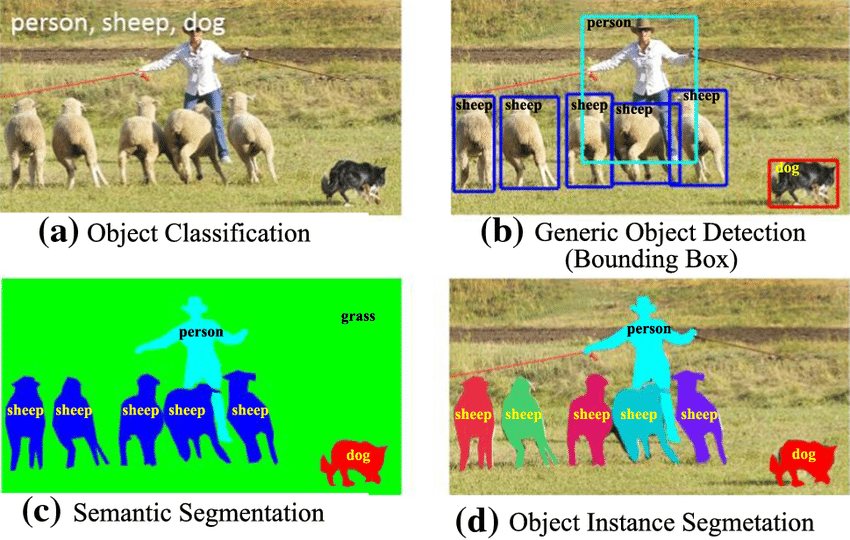
\includegraphics[width = 0.5\textwidth]{Recognition-problems-related-to-generic-object-detection-a-image-level-object.png}
    \caption{Résultat de différentes méthodes de vision par ordinateur pour une même image.\hl{vérifier droits d'auteurs} Source: \cite{Minaee:ImageSegmentation:2022}}
    \label{fig:computer_vision_problems}
  \end{figure}
  Les processus varient aussi dans leur résultante. Tandis que les modèles de segmentation pure feront une affectation de la même couleur à plusieurs objets d'un même type, la segmentation d'instance rend le processus de post traitement des raster plus simple en donnant une couleur différente à chaque instance d'un même type d'objet. Cette dernière propriété a le mérite de potentiellement faciliter le post traitement des résultats.
  \subsection{Algorithmes de segmentation sémantique basés sur la convolution}

  \subsubsection{U-Net}
    U-net a initiallement été développé comme méthode de segmentation d'imagerie médicale par \textcite{Ronneberger:UNetConvolutional:2015}. Dans son implémentation initiale, le diagramme du réseau est donné à la figure \ref{fig:unet_arch}.
    \begin{figure}[!h]
      \centering
      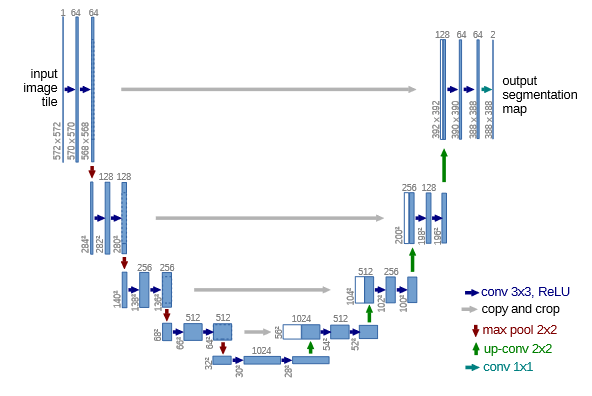
\includegraphics[width= 0.8 \textwidth]{unet_architecture.png}
      \caption{Architecture de réseau U-net \parencite{Ronneberger:UNetConvolutional:2015}}
      \label{fig:unet_arch}
    \end{figure}
    L'architecture peut être séparée en deux grandes phases. À gauche, il ya une phase d'encodage qui est constituée de 4 sous blocs. Chaque sous bloque est constituée de deux opérations de convolution 3x3 et d'activation \ac{ReLu} suivi d'un sous-échantillonage utilisant max-pool pour augmenter le niveau d'abstraction, créer un carte de caractéristiques de plus en plus grossière et abstraite. Au niveau d'abstraction le plus haut, une carte de caractéristique de 32x32 est créée au goulot d'étranglement du réseau. La partie de droite constitue le décodeur. Dans cette phase, la carte des caractéristiques des niveaux d'abstraction supérieurs est sur échantillonée, concatennée avec le résultat de convolution, puis passe par une opération de double convolution. Le processus est repété jusqu'à revenir à la résolution de départ pour générer le masque de segmentation de l'image avec un convolution 1x1 finale. Plusieurs implémentations ont été trouvées qui créaient des masque de la même taille que l'image d'origine en utilisant du garnissage de zéro 
  \subsubsection{Dense U-Net}

  \subsubsection{DenseLabV3+}
  \subsection{Algorithmes de segmentation d'instance basés sur la convolution}
  La première est la segmentation sémantique qui consiste à séparer des pixels dans une image par classe. La deuxième est la segmentation d'instance. Cette dernière reconnait des objets, le classifie et en extraie le contour. \textcite{He:MaskRCNN:2018} est l'article original sur la méthode qui a par la suite été adapté dans un contexte de reconnaissance SIG \parencite{Pesek:MaskRCNN:2018} ou pour la reconnaissance automatique de terrains sportifs pour réinjecter les polygones directement dans \ac{OSM} \parencite{Remillard:JremillardImagestoosm:2024}.\par
  \textcite{Fritz:InstanceSegmentation:2020} développe plusieurs estimés de segmentation d'instance pour des bâtiments à l'aide de deux modèles. Le premier est celui cité plus haut\parencite{He:MaskRCNN:2018} tandis que le deuxième est un modèle de segmentation d'image modifié pour segmenter les instances \parencite{Iglovikov:TernausNetV2Fully:2018} une fois la segementation d'image complétée
  \subsection{Algorithmes de segmentation sémantique basée sur les transformeurs}
  \subsection{Algorithmes de segmentation d'instance basés sur les transformeurs}
  \subsection{Jeux de données disponibles à l'entrainement}
    Deux enjeux sont critiques au succès d'un projet d'apprentissage machine. La présence d'un modèle adapté à la tâche en cours et la présence d'un jeu de donnée annoté qui peut être utilisé pour ajuster les poids initiaux du modèle pour permettre de modifier les poids du modèle et permettre de l'appliquer à de grands ensembles de données. Le tableau suivant résumera les jeux de données actuellement disponibles pour la segmentation sémantique en milieu urbain:
    \begin{table}
      \centering
         \begin{tabular}{l p{0.2\textwidth} l p{0.3\textwidth}  p{0.2\textwidth} l} 
          \hline
          Nom & Origine & $N_{classes}$ & Classes pertinentes au stationnement & Point de vue\\
          \hline
          CNRParkEXT & \cite{Amato:DeepLearning:2017} & 2 & Places occupées, places libres & Caméra de surveillance \\
          PKLot & \cite{deAlmeida:PKLotRobust:2015} & 2 & Places occupées, places libres & Caméra de surveillance \\
          APKLot & \cite{Hurst-Tarrab:RobustParking:2020} & 1 & Grappes & Imagerie satellite\\
          Skyscapes & \cite{Azimi:SkyScapesFineGrained:2019} & 31 & Aires pavées, aires non-pavées & Orthophotos\\
          Grab-PkLot & \cite{Yin:ContextenrichedSatellite:2022} & 1 & Aires de stationnement & Orthophotos\\
          \hline
        \end{tabular}
        \caption{Jeux de données annotés de segmentation sémantique en milieu urbain}
        \label{tab:jeux_donnees_segmentation_urbain}
    \end{table}
    \FloatBarrier